\noindent
\begin{slikaDesno}{fig/int_fb.pdf}
\PID У систему са слике употребљени су идеални
блокови за интеграљење и суматори. Улаз система  
је континуалан сигнал $x = x(t)$ a излаз је 
континуалан сигнал $y = y(t)$. 
\end{slikaDesno}
\begin{enumerate}[label=(\alph*)]
    \item Описати 
    систем одговарајућом диференцијалном једначином,
    \item одредити импулсни одзив тог система,  $h(t)$, и
    \item испитати стабилност тог система
    у \textit{BIBO} смислу.
\end{enumerate}
% %
% \begin{figure}[ht!]
%     \centering
%     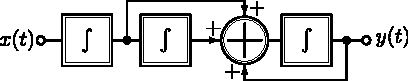
\includegraphics{fig/int_fb.pdf}
%     \caption{}
% \end{figure}

\vspace*{2mm}

\textsc{\underline{Резултат}} 
(а) $({\rm D}^3 - {\rm D}^2) y(t) = 
({\rm D} + 1) x(t)$, 
\quad
(б) $h(t) = 
\bigl(
-2-t+2{\rm e}^t
\bigr)
\,\uu(t)$.
\quad
(в) Систем није 
\textit{BIBO}
стабилан.
